\documentclass[]{scrartcl}


\usepackage[ngerman]{babel}
\usepackage{default}
\usepackage[utf8]{inputenc}
\usepackage{graphicx}


\usepackage{amsmath}
\usepackage{amssymb}
\usepackage{amsthm}

\newtheorem{definition}{Definition}[section]
\newtheorem{satz}[definition]{Satz}
\newtheorem{bsp}[definition]{Beispiel}

%opening
\title{Postsches Korrespondenzproblem}
\author{Soeren Berken-Mersmann}

\begin{document}

\maketitle

\begin{abstract}

\end{abstract}

\section{Einleitung}

\section{Postsches Korrespondenzproblem}

	\subsection{Definition}
	
		Das Postsches Korrespondenzproblem (PKP) ist benannt nach Emil Leon Post. Es handelt sich um ein konstruiertes Problem aus der theoretischen Informatik und ist folgendermaßen definiert:
		
		\begin{definition}
			Gegeben sei eine endliche Menge an Wortpaaren $K = ((x_1, y_1), ..., (x_k, y_k))$, über dem Alphabet $\Sigma$ mit $x_i, y_i \in \Sigma$. Gibt es eine Folge von Indizes $i_1, i_2, ..., i_n \in {1, 2, ..., k}, n \geq 1$, so dass $x_{i_1},x_{i_2}, ... x_{i_n} = y_{i_1}, y_{i_2}, ..., y_{i_n}$?
		\end{definition}
		
		Das Problem lässt sich besser Visualisieren als Menge von Dominosteinen: Ein Dominostein besteht jeweils aus einem oberen ($x_i$) und unteren ($y_i$) Symbol aus dem Alphabet $\Sigma$. Die Fragestellung lautet nun, ob es eine Reihenfolge gibt in der die Dominosteine so aneinandergereiht werden können, dass oben und unten die selbe Symbolfolge entsteht. Dabei darf jeder Dominostein mehrfach verwendet werden. Diese Arbeit wird daher eine Schreibweise verwenden, die diese Visualisierung widerspiegelt.
	
	\subsection{Beispielinstanzen}
		
		Dieser Abschnitt wird an Hand von drei Beispielen zeigen, dass die Lösung des PKPs nicht trivial ist.

		\begin{bsp}
			\label{bsp-pkp1}
			Die Menge an Wortpaaren $K$ sei gegeben mit: \[K = \left\lbrace \begin{bmatrix}
					1 \\ 111
				\end{bmatrix}
				\begin{bmatrix}
					10111 \\ 10
				\end{bmatrix}
				\begin{bmatrix}
					10 \\ 0
				\end{bmatrix}\right\rbrace \]
				Die Lösung des PKPs lässt sich mit der Indexfolge $I_1 = (2, 1, 1, 3)$ angeben, so ergibt sich die Lösung:
				\[K_{I_1} = \begin{bmatrix}
								10111 \\ 10
							\end{bmatrix} \begin{bmatrix}
								1 \\ 111
							\end{bmatrix} \begin{bmatrix}
								1 \\ 111
							\end{bmatrix} \begin{bmatrix}
								10 \\ 0
							\end{bmatrix}\]
		\end{bsp}
		
		Das Beispiel \ref{bsp-pkp1} zeigt, dass es Instanzen des PKPs gibt für die sich eine Lösung finden lässt. Darüber hinaus handelt es sich um ein einfaches Beispiel, bei dem man mit ein wenig Knobelei selbst auf die Lösung kommen kann. Mit Hilfe von zwei weiteren Beispielen wird gezeigt, dass es sowohl weitaus komplexere Probleminstanzen gibt, die sich nicht mehr mit einem scharfen Blick lösen lassen (s. Beispiel \ref{bsp-pkp2}), als auch Fälle in denen es keine Lösung für das PKP gibt (Beispiel \ref{bsp-pkp3}).
		
		\begin{bsp}
			\label{bsp-pkp2}
			Die Instanz des PKPs sei gegeben mit der Menge an Wortpaaren $K$:
			\[K = \left\lbrace \begin{bmatrix}
						001 \\ 0
					\end{bmatrix}
					\begin{bmatrix}
						01 \\ 011
					\end{bmatrix}
					\begin{bmatrix}
						01 \\ 101
					\end{bmatrix}
					\begin{bmatrix}
						10 \\ 001
					\end{bmatrix}\right\rbrace \]
			Und ihre kürzeste Lösung ist $I_1$ mit insgesamt 66 Elementen:
			\begin{align*}
				I_1 = (2, 4, 3, 4, 4, 2, 1, 2, 4, 3, 4, 3, 4, 4, 3, 4, 4, 2, 1, 4, 4, 2, 1, 3, 4, 1, 1, 3, 4, 4, 4, 2, 1,\\ 2, 1, 1, 1, 3, 4, 3, 4, 1, 2, 1, 4, 4, 2, 1, 4, 1, 1, 3, 4, 1, 1, 3,
					1, 1, 3, 1, 2, 1, 4, 1, 1, 3 )
			\end{align*}
		\end{bsp}
		\begin{bsp}
			\label{bsp-pkp3}
			Die Instanz des PKPs sei gegeben mit der Menge an Wortpaaren $K$:
			\[K = \left\lbrace \begin{bmatrix}
						10 \\ 101
					\end{bmatrix}
					\begin{bmatrix}
						011 \\ 11
					\end{bmatrix}
					\begin{bmatrix}
						101 \\ 011
					\end{bmatrix}\right\rbrace \]
			Das einzige Wortpaar mit dem angefangen werden kann ist das erste. Darauf muss zwangsläufig das dritte Paar folgen.  Da nun die untere Wortfolge der oberen um ein Symbol vorauseilt, passt erneut nur das dritte Paar. Folglich kann die $y$-Folge nie aufschließen, und diese Instanz des PKPs hat keine Lösung.
			\[
			\begin{bmatrix}
						10 \\ 101
					\end{bmatrix} 
					\begin{bmatrix}
						101 \\ 011
					\end{bmatrix}
					\begin{bmatrix}
						101 \\ 011
					\end{bmatrix} ...
			\]
		\end{bsp}

\section{Beweis der Nichtberechenbarkeit}
	In diesem Kapitel soll die Nichtentscheidbarkeit des PKPs bewiesen werden. Dazu wird das Halteproblem für Turingmaschinen zu Hilfe genommen.

	\subsection{Simulation einer Turingmaschine}
		Dazu soll zuerst gezeigt werden, wie mit Hilfe des PKPs eine Turingmaschine simuliert werden kann. Dabei wird eine Turingmaschine mit einem beidseitig unendlichem Band und dem Bandalphabet $\varGamma = {0,1}$ verwendet, ohne die Allgemeinheit zu beschränken. Um die Turingmaschine mit Hilfe des PKPs simulieren zu können, muss zuerst ihr Rechenweg formalisiert werden. 
		
		
		\paragraph{Der Rechenweg einer Turingmaschine}
			Der Rechenweg beschreibt dabei die von der Turingmaschine durchlaufenen Zustände\footnote{Mit Zuständen wird der gesamte Zustand der Turingmaschine gemeint, und nicht der Zustand des Turingprogramms. Der Verständlichkeit halber wird dieser Programmzustand im weiteren als interner Zustand bezeichnet.} vom Beginn der Berechnung bis zu einem (möglichen) Endzustand. Der Rechenweg ist folglich eine Folge von Zuständen.
			
			Der Zustand einer Turingmaschine lässt sich mit den folgenden Punkten vollständig beschreiben (Vgl. Abbildung \ref{img-turingsnapshot}):
			\begin{figure}
				\centering
				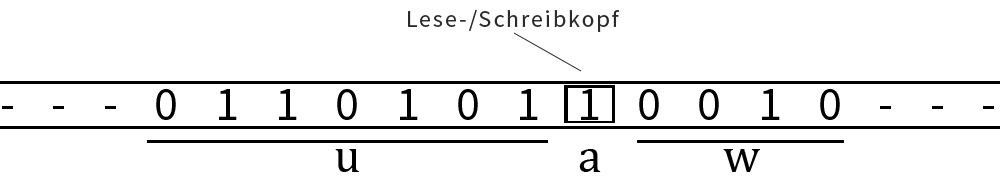
\includegraphics[width=0.85\linewidth]{../abbildungen/turing-snapshot}
				\caption{Illustration des Zustands einer Turingmaschine mit beidseitig unendlichem Band.}
				\label{img-turingsnapshot}
			\end{figure}
			
			\begin{itemize}
				\item Linkskontext: $u$
				\item Interner Zustand: $q$
				\item Gelesenes Symbol: $a$
				\item Rechtskontext: $w$
				\item Position des Lese- und Schreibkopfes
			\end{itemize}
			
			\begin{satz}
			Somit lässt sich der Zustand $Q_t$ einer Turingmaschine zum Zeitpunkt $t$ durch die Folge $Q_t = u_tq_ta_tw_t$ darstellen. Dabei ist die Position des Lese- und Schreibkopfes durch die Position des internen Zustands innerhalb der Folge $Q_t$ kodiert. Folglich lassen sich das gelesene Symbol $a_t$ und der Rechtskontext $w_t$ auch zusammenfassen.
			\end{satz}
			
			\begin{satz}
			Den Rechenweg einer Turingmaschine können wir als die Folge von Zuständen $Q_0, ..., Q_n$ vom Startzeitpunkt $t = 0$ bis zum Endzeitpunkt $t = n$ bei dem die Turingmaschine einen der Endzustände erreicht hat.
			\end{satz}
		
		\paragraph{Simulation mit Hilfe des PKPs}
			Wir benötigen nun Regeln, um aus dem formalisierten Rechenweg einer Turingmaschine eine Instanz des speziellen PKPs\footnote{Das spezielle PKP hat die Einschränkung, dass das Startwortpaar bereits gegeben ist.} konstruieren zu können. Das Ziel ist es, dass die Instanz des PKPs genau dann eine Lösung hat, wenn die damit simulierte Turingmaschine terminiert. Diese Konstruktionsregeln sehen folgendermaßen aus:
			\begin{definition}
				\label{def-simulation}
				Für eine gegebene Turingmaschine $M = (Q, \Sigma, \varGamma, \delta, q_o, \varepsilon ,Q_f)$ mit der Menge der inneren Zustände $Q$, dem Eingabealphabet $\Sigma$, dem Bandalphabet $\varGamma$, dem (inneren) Startzustand $q_0$, dem leeren Symbol $\varepsilon$ sowie der Menge an (inneren) Finalzuständen $Q_f$ kann mit nachfolgenden Regeln eine Instanz eines PKPs konstruiert werden, so dass dieses genau dann eine Lösung hat, wenn die Turingmaschine für das Eingabewort $w$ in einen Endzustand gelangt.
				\begin{tabbing}
					XXXX \= XXXXXXX \= X \kill
						\textbf{1. Anfangsregel}\\
							\> \textbullet $\begin{bmatrix}\sharp\sharp q_0w\sharp \\ \sharp\end{bmatrix}$ \> (Startwortpaar)\\
						\textbf{2. Kopierregel}\\
							\> \textbullet$\begin{bmatrix} a \\ a \end{bmatrix}$ \> für alle $a \in \varGamma \cup \left\lbrace \sharp \right\rbrace$\\
						\textbf{3. Überführungsregeln}\\
							\> \textbullet$\begin{bmatrix} cq' \\ qa \end{bmatrix}$ \> falls $(qa \rightarrow q'cR) \in \delta$, für $q \in Q, a \in \varGamma$ \\
							\> \textbullet$\begin{bmatrix} q'bc \\ bqa \end{bmatrix}$ \> falls $(qa \rightarrow q'cL) \in \delta$, für $q \in Q, a \in \varGamma$\\
						\textbf{4. Aufholregeln}\\
							\> \textbullet$\begin{bmatrix} q \\ aq \end{bmatrix}$ \> für alle $a \in \varGamma$ und $q \in Q_f$\\
							\> \textbullet$\begin{bmatrix} q \\ qa \end{bmatrix}$ \> für alle $a \in \varGamma$ und $q \in Q_f$\\
						\textbf{5. Abschlussregel}\\
							\> \textbullet$\begin{bmatrix} \sharp \\ q\sharp\sharp\end{bmatrix}$ \> für alle $q \in Q_f$

				\end{tabbing} 
			\end{definition}
			Anmerkung: Die hiermit simulierte Turingmaschine bewegt ihren Lese- und Schreibkopf in jedem Rechenschritt entweder nach Rechts oder nach Links. Der Übersichtlichkeit halber wurden zusätzliche Regeln die für den Fall benötigt werden, dass der Kopf den Rand des beschriebenen Teils erreicht, weggelassen. Diese können in WEGENER EINFÜGEN nachgelesen werden.
			
			Die Simulation des Rechenwegs der Turingmaschine kann man sich folgendermaßen visualisieren: Man hat zwei übereinander stehende Wortfolgen, bei der das untere Wort jeweils die bereits abgeschlossenen Rechenschritte darstellt, und das obere entsprechend zusätzlich den darauf folgenden Rechenschritt abbildet. So eilt das untere Band dem oberen Band so lange hinterher, bis die Aufholregeln eingesetzt werden können, sprich die Turingmaschine einen Finalzustand erreicht hat. Diese Aufholregeln ermöglichen es nun dem unteren Wort Schritt für Schritt aufzuholen, bis nur noch das - aus der Abschlussregel konstruierte - Wortpaar verwendet werden kann, und es das obere Wort einholt. Damit hat diese PKP Instanz genau dann eine Lösung wenn die Turingmaschine einen Finalzustand erreicht. Die Konstruktionsregeln aus Definition \ref{def-simulation} lassen nur unter dieser Bedingung ein Aufholen des unteren Wortes zu.
			
			Das folgende Beispiel dient der Verdeutlichung des Simulationsablaufs:
			\begin{bsp}
				Gegeben sei eine Turingmaschine $M$, die sich derzeit im Zustand $Q_t = 0110101q_2100010$ befindet. Durch die Anwendung der Regel $q_21 \rightarrow q_11R$ gelangt sie in den Folgezustand $Q_{t+1} = 01101011q_100010$. Der darauf folgende Rechenschritt soll nun mit Hilfe des nach Definition \ref{def-simulation} konstruierten PKPs simuliert werden. Dabei findet folgende Regel Anwendung: $q_10\rightarrow q_11R$
				\begin{tabbing}
				XXXX \= XX \= X\kill
				\>\textbullet Ausgangslage\\
				\>\> $...0110101q_2100010\sharp01101011q_100010\sharp$\\
				\>\> $...0110101q_2100010\sharp$\\
				\>\textbullet Anwendung der Kopierregel\\
				\>\> $...0110101q_2100010\sharp01101011q_100010\sharp0$\\
				\>\>$ ...0110101q_2100010\sharp0$\\
				\>\textbullet Anwendung der Kopierregel\\
				\>\> $...0110101q_2100010\sharp01101011q_100010\sharp01$\\
				\>\>$ ...0110101q_2100010\sharp01$\\
				\>\textbullet Mehrfache Anwendung der Kopierregeln\\
				\>\> $...0110101q_2100010\sharp01101011q_100010\sharp01101011$\\
				\>\>$ ...0110101q_2100010\sharp01101011$\\
				\>\textbullet Überführungsregel zu $q_10\rightarrow q_11R$\\
				\>\> $...0110101q_2100010\sharp01101011q_100010\sharp011010111q_1$\\
				\>\>$ ...0110101q_2100010\sharp01101011q_10$\\
				\>\textbullet Erneute Mehrfache Anwendung der Kopierregeln\\
				\>\> $...0110101q_2100010\sharp01101011q_100010\sharp011010111q_10010\sharp$\\
				\>\>$ ...0110101q_2100010\sharp01101011q_100010\sharp$\\
				\end{tabbing}
				Somit erhalten wir den nachfolgenden Turingrechenschritt durch obenstehende Simulation mit $Q_{t+2} = 011010111q_10010$.
			\end{bsp}

	\subsection{Reduktion des Halteproblems}
	
		Wie bereits im vorangegangen Abschnitt beschrieben, hat die nach Definition \ref{def-simulation} konstruierte Instanz des Postschen Korrespondenzproblems nur dann eine Lösung, wenn die Turingmaschine $M$ mit der Eingabe $w$ einen Finalzustand erreicht, sprich terminiert. Das Halteproblem für Turingmaschinen besagt allerdings, dass es nicht entscheidbar ist, ob eine Turingmaschine für eine beliebige Eingabe terminiert. Damit ist das PKP ebenfalls nicht entscheidbar.
		
		\begin{satz}
		Sei $M$ eine Turingmaschine und $w$ ihre Eingabe, so lässt sich das Halteproblem für Turingmaschinen durch die Übergangsfunktion $f$ (nach Definition \ref{def-simulation}) auf das PKP reduzieren:
		\[X_{Halte} (M, w) \Leftrightarrow X_{PKP}(f(M, w))\]
		Damit ist bewiesen, dass das PKP ebenfalls nicht berechenbar ist.
		\end{satz}

\section{Beweise mit Hilfe des PKPs}

	\subsection{Eindeutigkeitsfrage}

	\subsection{Äquivalenzproblem}

\end{document}
